\documentclass[../main/main.tex]{subfiles}

\newdate{date}{04}{06}{2020}

\begin{document}

\section{Lecture 21}
 \displaydate{date}. Compiled:  \today. Rachele 

\renewcommand\vec{\mathbf}

\subsubsection{Slide 349}


\begin{figure}[h!]
\centering
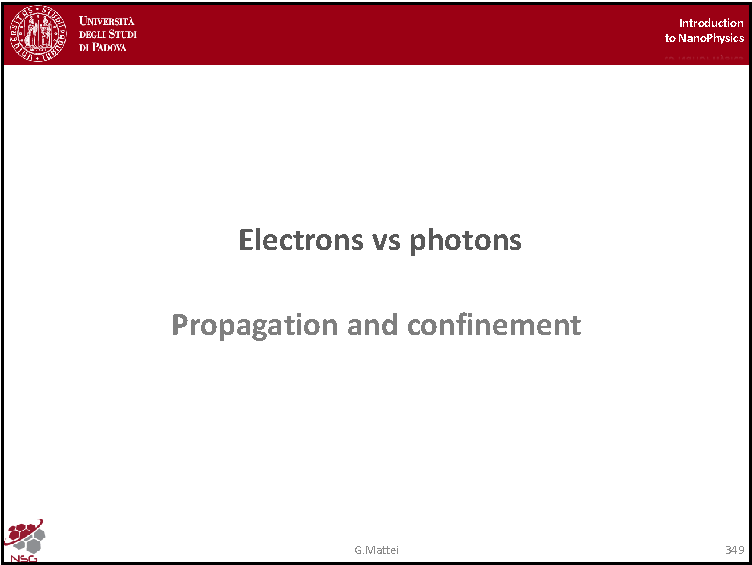
\includegraphics[page=1,width=0.9\textwidth]{../lessons/pdf_file/21_lesson.pdf}
\end{figure}


In this lesson I’ll discuss new problems like propagation and confinement of electrons and photons and some analogies between them.

We worked a lot with photons and and we saw how they interact with electrons to create polarization for the surface plasmons in metallic nanoparticles, but it's interesting to see which are the rules of confinement and control of the propagation, because they are the base of the design of devices to control light and matter at the nanoscale to obtain new functionalities. 


\newpage


\subsubsection{Slide 350}

\begin{figure}[h!]
\centering
\includegraphics[page=2,width=0.9\textwidth]{../lessons/pdf_file/21_lesson.pdf}
\end{figure}

If we want to describe light in a classical way, we have to use the Maxwell Equations.
They are written by specifying the electric and magnetic field, the free current and the charge density.
There are links between those quantities and it’s easy to obtain the continuity equation for the current and the equations for $\vec{D}$, $\vec{E}$ and the polarization $\vec{P}$ and $\vec{H}$, $\vec{B}$ and the magnetization $\vec{M}$. 
Other important relations define the relative permittivity $\epsilon$ and permeability $\mu$. They are related to electric $\chi_e$ and magnetic susceptibility $\chi_m$.
All those relations are the ground base of the electrodynamic description of materials.

Finally there is a link between the dielectric function $\epsilon$ and the complex refractive index $n$. 
The real part $\epsilon_1$ is the difference of the squares of the real and imaginary part of the complex refractive index; the imaginary part $\epsilon_2$ is the product of the two.
So we can have a very complete description of the material properties, once we are able to solve those equations.

If we search for plane wave solutions, we have a very simple harmonic dependence on time and this simplifies the derivative operator, which is a multiplicative operator with $-i \omega$ with respect to the argument.
In general also the nabla operator is equivalent to $\vec{K}$ wavevector, because whenever you do a gradient or a curl, you have a sort of multiplication by $\vec{K}$ vector. 


\newpage 

\subsubsection{Slide 351}

\begin{figure}[h!]
\centering
\includegraphics[page=3,width=0.9\textwidth]{../lessons/pdf_file/21_lesson.pdf}
\end{figure}


If we solve Maxwell equations with plane wave solutions, they simplify in this form.
Of course we can derive the Helmholtz equations by taking the curl of the first equations and using the standard identity of vectorial calculus.
Those equations are in general non homogeneous, because they involve the free current density or the free charge density. 
Instead we consider the homogeneous case, in which there are no free current nor charges. 
We can solve those equations for any domain in our system (even if we are not in a homogeneous medium, like for instance a nanoparticle embedded in medium or in a more complicated structure).

If we want to solve the Helmholtz equation for each domain (labelled by $i$), we need to apply suitable boundary conditions. They are calculated at the boundary between two domains imposing the continuity of the tangential component of the electric field and the development of a surface current density for the tangential component of $\vec{H}$ field; with a surface charge density polarisation we have the continuity for the normal component to the surface of the displacement vectors and finally we impose continuity for the $\vec{B}$ vector.
Normally the surface current density and the surface charge density are 0, so the tangential component of $\vec{E}$ and $\vec{H}$ are continuous, whereas the normal component of $\vec{D}$ and $\vec{B}$ are continuous.
So we can match all the solutions that we find for each specific domain, in order to have a global solution which is valid for all domains.

\newpage

\subsubsection{Slide 352}

\begin{figure}[h!]
\centering
\includegraphics[page=4,width=0.9\textwidth]{../lessons/pdf_file/21_lesson.pdf}
\end{figure}

If we want to solve the homogeneous Helmholtz equation, we arrive at this equation for the dispersion law of our material ($\vec{K}$ is the wavevector of the planewave that we search for a specific solution).
For transverse wave we have $\vec{K} \cdot \vec{E} =0$, because we have the tranversality condition, which is the usual condition for propagating waves. 
This way we can switch off the first term and find the usual dispersion relation, in which the wavevector in the material is related to $\omega /c$ (=k vector of photons in vacuum) times the relative dielectric function of the material.

We can also search for solution for longitudinal waves, but in this case the first two terms are equal so the only solution is $\epsilon=0$. This is exactly the condition for the onset of the volume bulk plasmon for a given material. We have longitudinal waves propagating because we have a coherent collective motion of electrons in our system.

\newpage

\subsubsection{Slide 353}

\begin{figure}[h!]
\centering
\includegraphics[page=5,width=0.9\textwidth]{../lessons/pdf_file/21_lesson.pdf}
\end{figure}

If we want to have a comparison of the properties of photons and electrons, we can be surprised by the analogies between the two particles, even if they are remarkably different at the microscopic level.

They differ for mass, charge and statistic but we can define for both of them an associated wavelength with the De Broglie relation.
For photons (classical description) we can write a scalar Helmholtz equation, that looks very similar to the Schroedinger equation which controls the stationary states for electrons (quantum mechanical particles). In this case we can write for the wavefunction the very same equation as the Helmholtz equation: we can make the analogy, $\vec{k}$ vector is controlled by the interaction potential. 

The free space solution of both eigenvalue equations is the plain wave. 
The interaction is controlled by $\epsilon$ for photons and its equivalent for electrons is the potential. Electron propagation is controlled by $V$ in the Schroedinger equation (note that $\epsilon$ in that equation is the eigenvalue of the Hamiltonian). 

There is a strong analogy that we can set between these two Helmholtz equations and so we can have all the properties of a typical quantum particle also for photons: similarly to the electron tunnelling (that is the exponentially decay probability when some particles penetrate a potential energy barrier with a height greater than the total energy of the particles, but thin enough to let them pass) we can obtain a photon tunnelling (it is an evanescent wave which propagates in the forbidden zone in which the wavevector becomes a complex value).

We can obtain a band structure for both: the crystalline band structures for electrons (derived by the regular array of the atoms on the lattice which produces the removal of degeneracy) and the very same effect for photons. We can build photonic crystals as the equivalent of a periodic modulation, not of the interaction potential, but of the dielectric function. So we can control exactly the propagation of photons by modulating the material similarly to what we do for electrons with atoms.

We can speak about cooperative effects: nonlinear optics, when there is a very strong electric field and the photons are interacting in a way that you cannot longer apply the superposition of fields, and similarly we have many body correlations for electrons in solid state physics (Cooper pairs in superconductivity,…). 

The classical description for photons and the quantum mechanical description for electrons are very similar with so many aspects, so we can use similar effects to describe propagation and confinement of both systems by suitably regulating the two parameters which control the material properties, that are the potential for electrons and the modulation of the dielectric functions for photons.

\newpage

\subsubsection{Slide 354}

\begin{figure}[h!]
\centering
\includegraphics[page=6,width=0.9\textwidth]{../lessons/pdf_file/21_lesson.pdf}
\end{figure}

Despite the analogies that we have seen for two particles, photons and electrons, their propagation and confinement are clearly different for many aspects. 
Let's see the dispersion law for photons and electrons in free space, which is the simplest medium you can imagine (homogeneous, linear,..).

For photons we have the very simple solution $\epsilon = 1$, we can write immediately the dispersion as $\omega=c k$ and the energy as $\epsilon = \hbar \omega$. The medium is non-dispersive in the sense that the phase velocity and group velocity are the same. The modulus of the phase velocity is $\omega / k$ and it can exceed the speed of light; on the contrary the group velocity, which is defined as the gradient of the $\omega$ with respect to $K$ vector, cannot exceed the speed of light, because the speed at which the information is transferred or the particle is moved or the centre of the particles (if we built a bunch of photons with wavevectors closed one to each other with a given dispersion around that value).
So we can confine and better localize photons in space and have a sort of uncertainty on the momentum definition.

For electrons the situation is similar: the solution of the Schroedinger equation for free-space has the energy proportional to $k^2$ (for photons it is proportional only to power 1 of $k$ vector). So in this case we can represent the energy in a one dimensional picture as a parabola centred at the origin of our system.
Even free space (vacuum) is dispersive for electrons, because the group velocity is the derivative of the energy and so it is two times the phase velocity. This is a remarkable difference between the two particles.

\newpage

\subsubsection{Slide 355}

\begin{figure}[h!]
\centering
\includegraphics[page=7,width=0.9\textwidth]{../lessons/pdf_file/21_lesson.pdf}
\end{figure}

The Snell law states that if $n_ 2$ is lower than $n_1$, the refracted ray will go far from the normal to the interface. 
With this simple consideration it’s easy to see that if we increase $\theta_1$, the refracted ray can be reflected to a higher angle till it reaches a direction parallel to the interface. That angle is called the critical angle and if we further increase the incident angle we will have a total internal reflection, that is a refraction no more in the external medium, but a confinement in the same medium.

This is at the base of the optical fibres, in which we have larger refractive index, surrounded by a lower refractive index (air in this case), so light can propagate within the medium provided that it enters at very low angle with respect to the interface (it propagates closely 90 degrees with respect to the normal to the interfaces). So we can obtain very easily a waveguide with this procedure.

If we want to calculate the critical angle we can put the angle $\theta_2 = \pi /2$ and invert the Snell law. For the pair silica-air pair the critical angle is around 43 degree, so if we enter with an angle larger than this value, we will stay within the silica fibre and be guided within that system.

The very same phenomenon happens when you are in the pool underwater and you look upstairs at a large angle and you cannot see outside water, whereas if you look straight in the perpendicular direction you see the sky.

\newpage

\subsubsection{Slide 356}

\begin{figure}[h!]
\centering
\includegraphics[page=8,width=0.9\textwidth]{../lessons/pdf_file/21_lesson.pdf}
\end{figure}


Now let’s look at the global confinement properties.
Consider $n_1 > n_2$, for photons we can have an optical planar waveguide, 1D confinement and photons free to propagate in the other two directions: this is like the quantum well for electrons, where they are confined in a lower potential with respect to the external potential. 

2D confinement is an optical fiber, a long cylinder with refractive index larger than the external one, so we can easily propagate light inside: this is exactly the quantum wire for electrons, in which we have confinement in 2 dimensions.

Finally we can have 3D confinement. If we are able to enter in a microsphere in which the refractive index is larger than air, we can trap light in that resonant optical cavity. The equivalent for electrons is the quantum dot, that is a system in which electrons are confined with all the three dimensions


\newpage

\subsubsection{Slide 357}

\begin{figure}[h!]
\centering
\includegraphics[page=9,width=0.9\textwidth]{../lessons/pdf_file/21_lesson.pdf}
\end{figure}


Let's see the analogies for 1D confinement for photons and electrons.
For photons consider an $n_1$ medium sandwiched between two $n_2$ medium. These are the transverse electric modes 0, 1, 2 of the solution of the Helmholtz equations. 

They resemble very closely the problem of the particle in a box for electrons, with 0 potential inside and infinite outside. In this case the wavefunction goes to zero at the boundary, there is no propagation outside.
Of course it's not exactly the same, but this is due to the infinite potential outside the box.
The solutions are the functions $\Psi_n(x)$, in which the wavevector and the spectrum of the energy are quantized. The most important result is that the spacing between two neighbouring levels goes with the inverse of the square of the length of the box, so the smaller is the box, the larger will be the separation in energy between two subsequent levels.


\newpage

\subsubsection{Slide 358}

\begin{figure}[h!]
\centering
\includegraphics[page=10,width=0.9\textwidth]{../lessons/pdf_file/21_lesson.pdf}
\end{figure}

We can push the analogy much better if we relax at the need of a closed solution (that is if we relax the request for an infinite external potential). With a finite confinement potential there is a spill out of electrons and we have exactly the very same solution as before for photons (an exponential decay solution on the region of the confinement potential).
The analogy is exact because the mathematics of the two equations are very similar.

\newpage

\subsubsection{Slide 359}

\begin{figure}[h!]
\centering
\includegraphics[page=11,width=0.9\textwidth]{../lessons/pdf_file/21_lesson.pdf}
\end{figure}

We have the very same effect: leakage and tunneling.

If we have a system with a waveguide, the solution at the border of the material will exponentially decay to zero in the forbidden zone, exactly similarly to the wavefunction of electrons, which goes exponentially faded in the forbidden zone, where the potential is larger than the energy of the particles.

Then we can have tunneling of photons, as well as tunneling electrons. In the case of electrons, their energy is lower than the energy of the barrier, so if it is of small thickness, the electrons have a chance to reach outside the barrier with an exponentially decay function within the barrier. So there is a propagation probability of electrons even on the other side of the barrier (with some attenuation).

The very same can occur for photons. If $n_1 > n_2$ and if light is entering with an angle larger than the critical angle, it’s the case of total internal reflection and light can’t enter the barrier.
But if on the other side there is another material, which refractive index is the same of the first one, and if we get closer (at the order of the wavelength) this interface to the first one, we can obtain the very same tunneling of photons, because the exponentially decay solution in the forbidden zone is sufficient to be coupled with the second material and to start the propagation with the very same initial direction of the photons inside the material in the first zone.

\newpage

\subsubsection{Slide 360}

\begin{figure}[h!]
\centering
\includegraphics[page=12,width=0.9\textwidth]{../lessons/pdf_file/21_lesson.pdf}
\end{figure}

This is at the base of the first multitouch screen.

In the photo on the right you can easily see the effect: if you illuminate the glass on the top and you touch with your fingers the surface, apparently your fingers are a source of light. This is due to the fact that the light is reflected exactly when your fingers are touching the glass, because the refractive index of your fingers is more or less the same (1.5) of the plexiglass one.
If you have the fingers position at a given point, you will see light scattered back as the light was coming from your fingers.

This is at the base of the multitouch screen, because if you use infrared light (which is not visible), light is confined within the material, until, when you touch the screen, you put a dielectric system, which has the very same refractive index and so there will be a scattering of light.
If you have an infrared camera beneath the screen, you will see that there was a finger touching in that specific area.

This is the mechanism of the earlier multitouch screens and they were all based on FTIR (frustrated total internal reflection).

\newpage

\subsubsection{Slide 361}

\begin{figure}[h!]
\centering
\includegraphics[page=13,width=0.9\textwidth]{../lessons/pdf_file/21_lesson.pdf}
\end{figure}

Let's see how we can obtain a perfect analogy of the electronic potential in a crystal for photons.
We discuss now the photonic crystal, that is an object which behaves for photons like an ordinary crystal for electrons.


\newpage

\subsubsection{Slide 362}

\begin{figure}[h!]
\centering
\includegraphics[page=14,width=0.9\textwidth]{../lessons/pdf_file/21_lesson.pdf}
\end{figure}

A photonic crystal is defined as a periodic structure in which we modulate periodically the dielectric function $\epsilon$ (function of $\omega$ and also of the coordinate $\vec{r}$ which varies periodically).
We can define a Bravais lattice defined by $\vec{R}$, so if we translate the spatial coordinates $\vec{r}$ respect to $\vec{R}$, we will obtain the very same dielectric function.
We can obtain this in different geometries: an example of 1D modulation is a model called Bragg Reflector; if we modulate in 2D we can have silicon pillars arranged in a exagonal closed packed geometry modulated by the air around; in 3D we can have a photonic crystal, if we stack a crystal of dielectric spheres we obtain a colloidal crystal with an optical modulation in 3D geometry, like the one in the third photo. 


\newpage

\subsubsection{Slide 363}

\begin{figure}[h!]
\centering
\includegraphics[page=15,width=0.9\textwidth]{../lessons/pdf_file/21_lesson.pdf}
\end{figure}

The easiest system to deal with is a 1D photonic crystal, in which we have modulation just in one dimension.
This is perfectly analogous to a Bragg reflector (so there is an analogy with the Bragg’s law for x-rays) and this geometry is widely used for obtaining perfect reflectors or antireflecting coatings in optical components.
In this particular case we have a modulation in one direction. Suppose we have an alternation of two different dielectrics materials with the period $a$ and we can obtain $\epsilon$ which is a real quantity.
Of course, if we have a periodicity in the real space by a given vector $a$, we can define a Bravais lattice and we have an automatically associated reciprocal space which is also a Bravais lattice with spacing $2 \pi / a$.
The sets of the integer multiple of $2 \pi / a$ constitute the entire set of reciprocal space vectors for the Bravais lattice in the reciprocal space.

In this simulation we have a stack made by 15 periods of two layers with different thickness (200 nm and 140 nm) and different refractive index (1.5 and 2.2, they could be for instance silica and titania). The angle of incidence is 25 degree with respect to the normal.
The graph shows the reflectivity as a function of $\lambda$ and we can see what is the region in which we have perfect reflection for that specific incident angle.
So we can optimize the devices for reflecting specifically the desired wavelengh.

This for the visible, but we can also obtain reflectors for x-rays, which are widely used in the parabolic mirror we have described in the x-ray diffraction experiment. The surface of the parabolic mirror is exactly coded in this strategy with a multilayer in which the reflectivity is maximum for the wavelength of 1.5 $\si{\angstrom}$.


\newpage

\subsubsection{Slide 364}

\begin{figure}[h!]
\centering
\includegraphics[page=16,width=0.9\textwidth]{../lessons/pdf_file/21_lesson.pdf}
\end{figure}

The theory of this multilayer goes exactly like the theory for the standard crystal for electrons. 
Whenever you have a periodicity, the solution of the wavefunction for electrons should be a Bloch wave. 
A Bloch wave is a plane wave with a modulation, in our case a plain wave with wavevector $k_0$ modulated by a periodic function with the periodicity of the crystal $a$. 
We can obtain the very same effect by constructing an infinite sum of plain waves with different $k$ vectors.


\newpage

\subsubsection{Slide 365}

\begin{figure}[h!]
\centering
\includegraphics[page=17,width=0.9\textwidth]{../lessons/pdf_file/21_lesson.pdf}
\end{figure}

The idea is to see what is the effect of the periodicity on the dispersion law.
Electrons in a periodic potential have a parabolic dispersion. Then, if we use the empty lattice model, so if we add periodicity without turning on the real potential, we can obtain the very same dispersion law by translating over the vectors in the reciprocal space (so the parabola centred in K describes the very same physics as the one centred in 0).
Since these two parabolas describe the very same state, at the crossing point there is a degeneracy which should be removed.
The way to remove it is turning on the periodic potential. If the potential is not that strong, we can use the perturbation theory. We can connect the two branches of this degenerate parabolas in order to obtain a gap whose magnitude is two times the modulus of the Fourier component of the potential calculated for that specific value of the reciprocal space vector K.
We have this degeneracy removal exactly at half of the length of the original reciprocal space vector K.

\newpage

\subsubsection{Slide 366} 

\begin{figure}[h!]
\centering
\includegraphics[page=18,width=0.9\textwidth]{../lessons/pdf_file/21_lesson.pdf}
\end{figure}

This ends up in the band structures. The first graph is in the extended zone: we removed degeneracy at each intersection by calculating the explicit form of the eigenvalues of the periodic Hamiltonian (the key ingredient is the periodicity of the potential U for the electrons).
The band gaps magnitude is controlled by the modulus of the Fourier transform of the potential in the reciprocal space.

\newpage

\subsubsection{Slide 367} 

\begin{figure}[h!]
\centering
\includegraphics[page=19,width=0.9\textwidth]{../lessons/pdf_file/21_lesson.pdf}
\end{figure}

Here we have an homogeneous system described by the empty lattice model: the dispersion law is a straight line centred in 0 and in every multiple of $\vec{G^*}$ (we can translate the very same dispersion law over any $\vec{G^*}$ vector of the reciprocal space vector, defined by $e^{i \vec{G} \cdot \vec{R} = 0}$, with $\vec{R}$ the Bravais lattice vector in the direct space).
Like before, there is a degeneracy at $\vec{G^*}/2$, at $\vec{G^*}$, and then again at $3\vec{G^*}/2$,… because in the reciprocal space the physics is invariant by translation over a multiple of the $\vec{G^*}$ vector.
So we need to remove the degeneracy at each point.  If we consider the $\Gamma$ point (the center of the Brillouin zone) and the $\vec{G^*}$ wavevector, we need to remove the degeneracy at $\vec{G^*}/2$.
If the $\vec{G^*}$ is the smallest reciprocal space vector (the one with magnitude $2\pi /R$), $\vec{G^*}/2$ is the boundary of the first Brillouin zone. 
This way we can recover a complete analogy with electrons.

We can proceed with the very same approach now if we have modulation of the dielectric function in our material within the period $a$.
We can immediately write $\epsilon$ in terms of the Fourier expansion over all the infinite set of the  $\vec{G}$ vector, the coefficient $\epsilon_\vec{G}$ are the Fourier transform of the dielectric function.
$V_c$ is the volume of the cell, in 1D is the length of the period, otherwise it would be the volume of the unit cell.
So we recover the band gap structure for electrons even for photons.


\newpage

\subsubsection{Slide 368}

\begin{figure}[h!]
\centering
\includegraphics[page=20,width=0.9\textwidth]{../lessons/pdf_file/21_lesson.pdf}
\end{figure}

The calculation goes straight forward. We need to solve the Helmholtz equation. 
$\epsilon$ is a periodic function of the coordinate, so we expand it  into Fourier series and we search for a very general solution for the electric field, which should obey the Bloch theorem, and we expand it into plain waves with amplitudes which are the unknowns of our system.

Since we are interested in removing the degeneracy at a particular value of the reciprocal space, where two of the light line intersect, we can consider that locally (that is around for instance $\vec{G^*}/2$ if we are considering the $\Gamma$ point and $\vec{G^*}$ vector) the best solution could be reasonably approximated by just summing 2 of this plain waves, that is the one centred at $\Gamma$ point ($\vec{G}=0$) and the other centred in $\vec{G^*}$.
Locally this is a very good approximation for the electric field.
If we substitute the two expansion, we have a very general master equation for the Helmholtz equation in the reciprocal space.
In this case applying $\nabla^2$ is putting a factor $k^2$ and we end up with the equation with the sum over $\vec{G’}$.  Then we can translate this equation by $\vec{G^*}$, this way we should obtain the same physics because the system is invariant with respect to the choice of the origin of the reciprocal space. 
So we can rewrite the very same equation by translating the $\vec{k}$ vectors by a given $\vec{G^*}$ vector.
We do not need to consider the entire set of $\vec{G’}$, but we can just sum the two vectors of relevance: $\vec{G’}=0$ and $\vec{G’}=\vec{G^*}$.
Doing this we end up with the last two equations with two unknowns: $\vec{A}(\vec{k})$ and $\vec{A}(\vec{k}-\vec{G^*})$.
All the other coefficients are known, because we know the explicit form of the dielectric function and so all the $\epsilon_\vec{G}$.

\newpage

\subsubsection{Slide 369}

\begin{figure}[h!]
\centering
\includegraphics[page=21,width=0.9\textwidth]{../lessons/pdf_file/21_lesson.pdf}
\end{figure}

We factorize for the unknown and we simplify the system.
The condition to have a non-trivial solution, in which the two unknowns are both 0, is to have the determinant of the coefficients which goes to 0 and so we have additional condition which is the dispersion law in our periodic system.
If we calculate the determinant and we set it equal to 0, we end up in this 4th order equation into the variable $\omega /c$.
Luckily it can be recast into ordinary 2nd order equation, so we can obtain a close solution for $\omega /c$ squared, which is the wavevector in vacuum squared.
The solution is strictly valid for $k$ values around the $\vec{G^*}/2$, where we have the degeneracy.


\newpage

\subsubsection{Slide 370}

\begin{figure}[h!]
\centering
\includegraphics[page=22,width=0.9\textwidth]{../lessons/pdf_file/21_lesson.pdf}
\end{figure}

If we want to calculate the solution at the degeneration, that is when $\vec{k} = \vec{G^*}/2$, we can simplify the previous expression for $\omega /c$ squared. 
$\epsilon_\vec{G^*} \cdot \epsilon_\vec{-G^*}$, due to the symmetry proprieties of the Fourier coefficient,  is the square modulus of the Fourier components of the refractive index.
So we end up with a formula for $\omega^2$, which tells us which are the variation of $\omega$ exactly calculated the at the intersection of the degenerate dispersion law.
We obtain a split of the two solutions into a non-degenerate solution.

If, like in the case represented in the graph, we have also inversion symmetry, all the Fourier components are real functions.
$\epsilon_0$ is the average of the dielectric functions in the two layers and $\epsilon_G$ when $G = 2 \pi /a $  is related to the difference between the dielectric functions.
If the two dielectric functions are equal, $\epsilon_G = 0$ and so we cannot remove the degeneracy because $\epsilon_G$  is involved in the solution expression and we go back into the degenerate case.

\newpage

\subsubsection{Slide 371}

\begin{figure}[h!]
\centering
\includegraphics[page=23,width=0.9\textwidth]{../lessons/pdf_file/21_lesson.pdf}
\end{figure}

In this case, with respect to the light line, we have a banding and a removal of the degeneracy exactly at the boundary of the first Brillouin zone: we have these two solutions or two bands.
At the boundary of the first Brillouin zone we have standing waves because we realise exactly the Bragg condition for perfect reflections (no propagation of information when the $k$ vector is at the value of $\pi /a$).
Exactly the same for electrons.

In this specific case we have two standing waves, if for instance $n_2 < n_1$, the standing wave in $n_2$ is the one with the higher energy and the modulus of the field is larger in the lower refractive index material.

The standing wave in the other branch of the dispersion law does not propagate information: it’s a stationary wave with maxima and minima confined in the high index material region.
So the square modulus which is proportional to the density of energy is mostly confined in the high index material, that is a normal result in electrodynamics (the lower configuration is obtained the when electric field is confined with the high refractive index material).

\newpage
\subsubsection{Slide 372}

\begin{figure}[h!]
\centering
\includegraphics[page=24,width=0.9\textwidth]{../lessons/pdf_file/21_lesson.pdf}
\end{figure}

At the boundary of the first Brillouin zone the group velocity goes to 0, because of course the derivative should be 0.
We can describe the acoustic branch for phonons, in this case for photons we have exactly the very same dispersion law, which is now non-degenerate.

\newpage

\subsubsection{Slide 373}

\begin{figure}[h!]
\centering
\includegraphics[page=25,width=0.9\textwidth]{../lessons/pdf_file/21_lesson.pdf}
\end{figure}

This is an example of a multilayer combining high dielectric materials: gallium arsenide with dielectric function $\epsilon_1 = 13$ and gallium aluminium arsenide with dielectric function $\epsilon_2 = 12$.
If we have just a perfect layer made with the same refractive index of gallium arsenide, we will have the linear dispersion law of the light line and degeneracy. 

Otherwise, if we add a tiny modulation by substituting some of the gallium atoms with aluminium atoms, so we have $\epsilon_1 = 13$ and $\epsilon_2 = 12$, we will have the onset of the photonic bandgap.

Moreover, if we increase the differences in the refractive index, for example by making a multilayer with alternating air ($\epsilon_2 = 1$) with gallium arsenide, we will have this very large photonic bandgap.
The magnitude of the degeneracy is related to the reflective index contrast.


\newpage

\subsubsection{Slide 374}

\begin{figure}[h!]
\centering
\includegraphics[page=26,width=0.9\textwidth]{../lessons/pdf_file/21_lesson.pdf}
\end{figure}

This is a representation of the electric field for the bands.
Normally we will have the lower energy configuration in the dielectric material with higher $\epsilon$. 
The bottom of the second band will see the electric field maximum and minimum in the lower dielectric layer.
If we look at the energy density, which is proportional to the square modulus of the electric field, we will see exactly what we have said before.

In the case of a stronger contrast we will have the very same effect, but now the shape of the field is different with respect to the purely sinusoidal wave on the left.


\newpage

\subsubsection{Slide 375}

\begin{figure}[h!]
\centering
\includegraphics[page=27,width=0.9\textwidth]{../lessons/pdf_file/21_lesson.pdf}
\end{figure}

We can obtain other interesting results computing the perturbation theory: it can be demonstrated that the bandgap can be constructed by integrating the energy density averaged over the refractive index contrast and integrated over the entire period of the system.
That is correct to the linear leading order in the refractive index contrast, so we can use the perturbation theory when $\Delta \epsilon \ll \epsilon $ and when the thickness of the first layer is much less than the period.



\clearpage

\end{document}